\chapter{Programmbeschreibung}
\label{chap:Programmbeschreibung}

\section{Pakete}
Die Hauptmodule des Programms sind nach dem Drei-Schichten-Modell aufgeteilt. Zudem ist für jedes Aufgabenfeld zunächst ein Interface deklariert, auf diese Weise bleibt das Programm erweiterbar. Gemäß .NET-Konvention beginnen die Namen der Interfaces mit einem \glqq I\grqq.
\newline
\begin{figure}
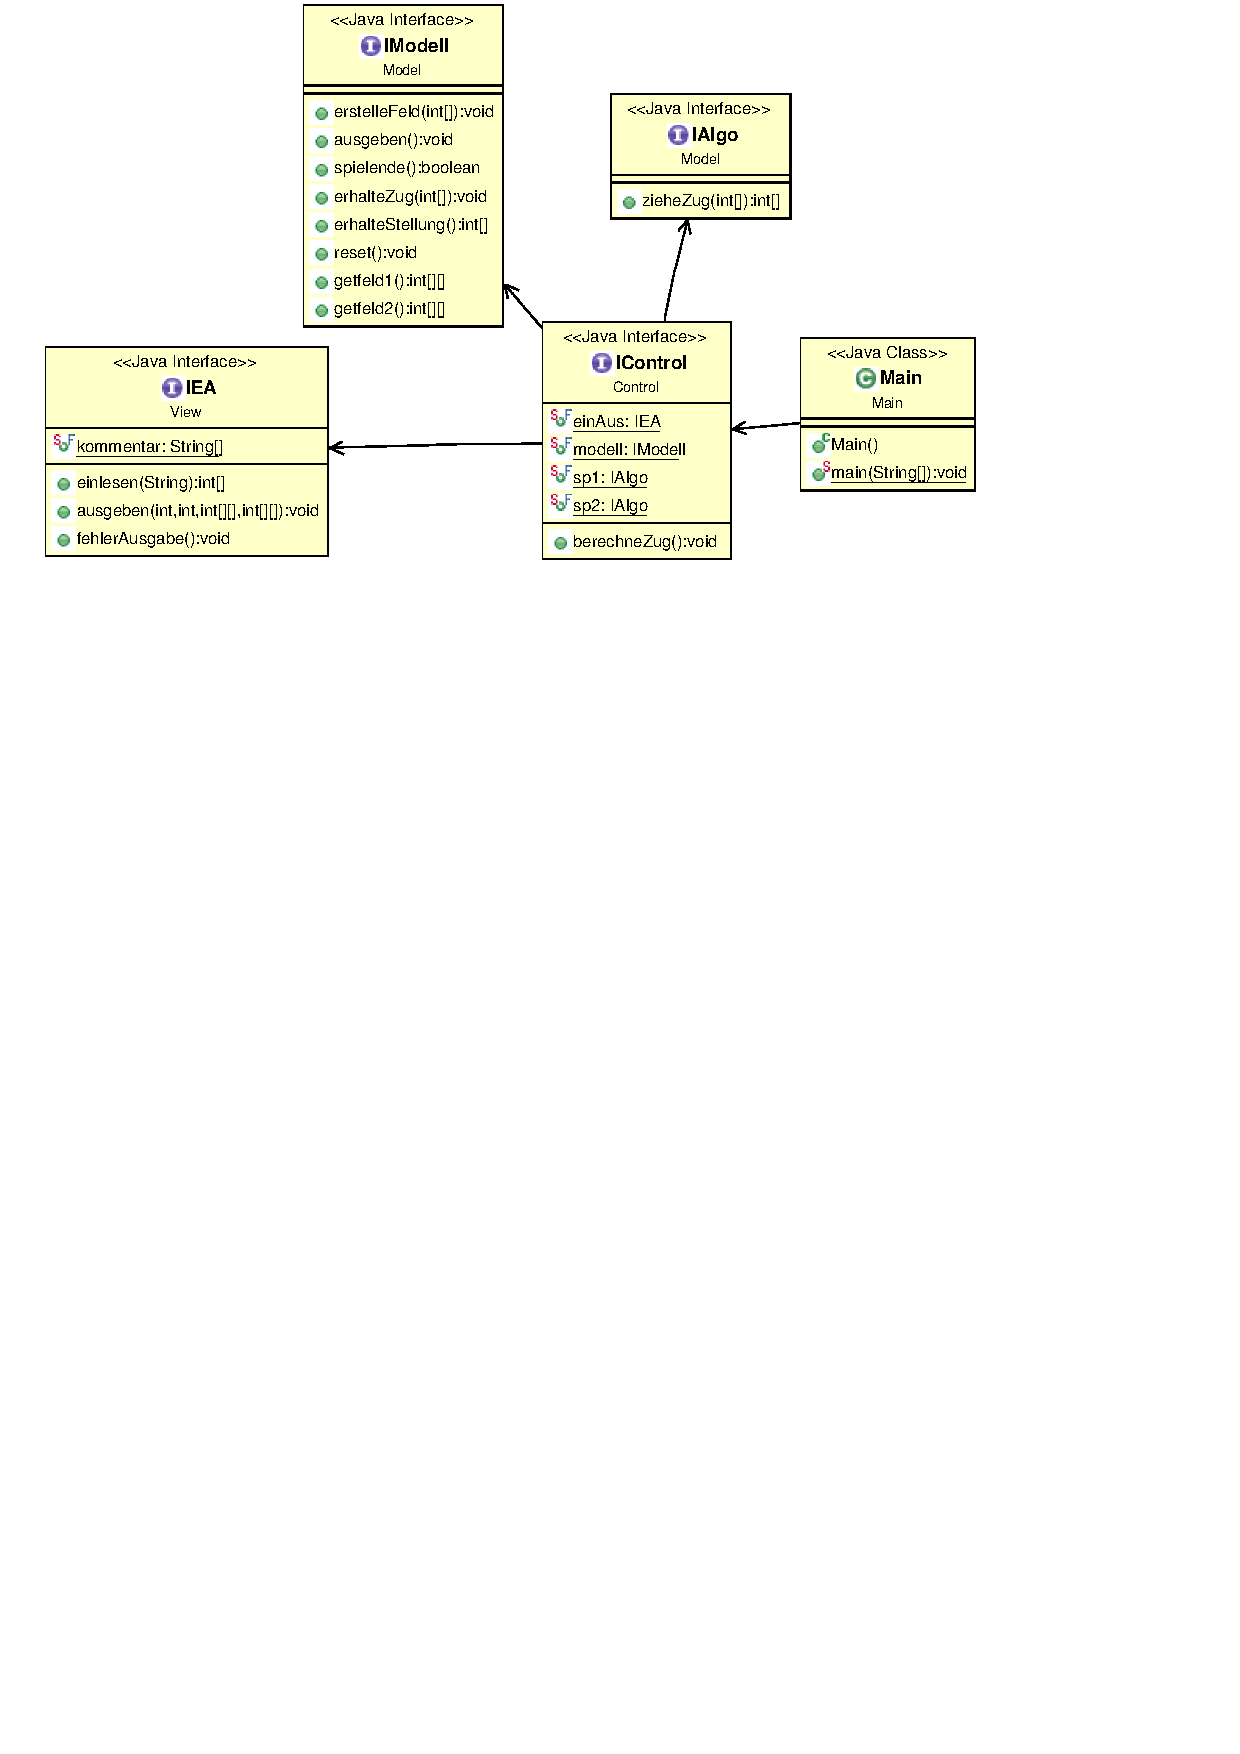
\includegraphics[viewport=50 50 0 0]{Diagramme/kontrolledia.pdf}
\end{figure}
